\section{Servicio DHCP}
	Es el protocolo de red que permite a un ordenador obtener una configuración de red (dirección IP y otros parámetros) automáticamente. Esta forma de obtener direcciones se denomina forma dinámica, frente a la forma estática, que es la que exige configuración por parte del usuario. La configuración dinámica de red sólo requiere de la existencia de un servidor DHCP en la red.
	
	\subsection{Antecedente}
		Tiene su origen en el protocolo BOOTP\footnote{Bootstrap Protocol, Protocolo de arranque} que se usaba antiguamente en las máquinas UNIX sin disco para que obtuviesen una dirección IP aún antes de arrancar cualquier sistema operativo. De hecho el modo que tenían estas máquinas sin disco de obtener el sistema operativo, era gracias a que después de obtener una IP, descargaban a través de un servidor TFTP \footnote{Trivial file transfer Protocol, Protocolo Trivial de Tranferencia de Ficheros} la imagen del sistema operativo. Este esquema de arranque se sigue utilizando hoy día en equipos que sólo funcionan como terminales, aunque suele usarse DHCP en vez de BOOTP.
	
	\subsection{Descripción del protocolo}
	El estándar original de 1993 del protocolo DHCP está definido a través de los siguientes documentos:
		\begin{itemize}
			\item{RFC 1531}
			\item{RFC 1532 Describe las opciones de configuración}
		\end{itemize}
	Actualizados en 1997 en los documentos:
		\begin{itemize}
			\item{RFC 2131}
			\item{RFC 2132}
		\end{itemize}	
		
Este protocolo abierto está implementado con una arquitectura cliente/servidor, que es la filosofía de los protocolos de la pila TCP/IP. El servidor escucha por el puerto 67 y el cliente por el 68 (el agente de retransmisión, relay agent, usa el 67 y el 68), usando UDP como protocolo de transporte.\\\\
El protocolo DHCP permite tres métodos de asignación de direcciones IP:

		\begin{itemize}
			\item Asignación estática: Consiste en que el administrador de la red configura el servidor DHCP para que asigne una IP fija a determinados equipos. Esto es posible gracias a que los clientes DHCP cuando hacen una solicitud de IP, se identifican (MAC u opción client identifier), lo que permite la asignación de una IP específica.
			\item Asignación dinámica: Con este método, el servidor DHCP dispone de uno o varios rangos (pools) de IP (al menos uno por cada segmento de red por el que se atienden peticiones de clientes), y cuando recibe una solicitud, éste selecciona una del pool adecuado y la asigna con un tiempo de alquiler (lease time), tiempo que se podrá prorrogar o en caso contrario, el cliente debe dejar de usar la IP, y comenzar una nueva solicitud.
			\item Asignación automática: La especificación del DHCP habla de este método, a través del cual el servidor DHCP asigna una IP como en la asignación dinámica, pero de forma permanente.
		\end{itemize}
		
		El protocolo DHCP define un conjunto de mensajes que se intercambian el cliente y el servidor DHCP para que el primero consiga una configuración de red sin intervención humana.\\\\
		El cliente, al conectarse a la red, necesita contactar con un servidor DHCP y conseguir una configuración de red. Para ello envía un mensaje de broadcast intentando localizar los potenciales servidores disponibles. Cuando el servidor DHCP recibe este mensaje, contesta con otro mensaje de broadcast, donde éste se identifica, y además oferta una IP libre, apropiada para el segmento de red del cliente, junto con otros parámetros necesarios. En este mensaje va también la dirección MAC del cliente, que de esta forma sabe que es para él. La dirección MAC del cliente le llegó al servidor en el primer mensaje.\\\\
		Una vez que la oferta llega al cliente, un nuevo mensaje de broadcast es enviado por el cliente, donde se solicita una IP y unos parámetros de red determinados, concretamente los ofertados por el servidor seleccionado. Este mensaje es necesario pues en la red puede haber varios servidores DHCP (por seguridad, por si un servidor falla, ya que es un servicio crítico; cada servidor serviría un rango distinto dentro de la misma subred) y este paso, es el que permite seleccionar a uno de ellos (normalmente el algoritmo de elección que se implementa consiste en coger al primero que llega), reutilizando los servidores rechazados, las IP ofertadas por ellos.\\\\
		Si el mensaje de requerimiento llega a tiempo al servidor, éste no habrá ofertado la IP a otro cliente, y por lo tanto, definitivamente la reserva para el cliente en cuestión, registrándola junto con su tiempo de alquiler, y a continuación, le envía un último mensaje de broadcast de aceptación, tras el cual, el cliente se configura y también, de forma local, registra la IP y el resto de parámetros, para un uso posterior.\\\\
		Cuando un equipo se reinicia, recupera su última configuración de red e intenta confirmar que puede utilizarla mandando un mensaje al servidor DHCP con todos los parámetros de red. Tras esto, el servidor comprueba si la IP puede utilizarla el cliente (puede haber sido asignada a otro cliente, el cliente puede haber sido movido de segmento de red, etc.), y en caso afirmativo, se lo confirma con un mensaje de aceptación, aunque existe la posibilidad de que el requerimiento sea rechazado y el cliente tenga que empezar el proceso desde el inicio, como si no hubiese tenido nunca una IP. Este último caso, puede ocurrir cuando un equipo se apaga en un segmento de red y se enciende en otro, de modo que el cliente intenta confirmar la configuración que tenía en el antiguo segmento de red y el servidor, al darse cuenta de que está en un segmento distinto, le rechaza la propuesta y el cliente comienza de nuevo desde el principio.\\\\
		En el caso anterior, si el cliente no recibiera respuesta del servidor, la decisión del cliente es la de configurarse con los antiguos parámetros de red que tenía.\\\\
		Un servidor DHCP deduce a qué segmento de red está conectado un cliente de dos formas:
			\begin{itemize}
				\item Si el cliente y el servidor están en segmentos distintos, un software, denominado agente de retransmisión (relay agent) debe reenviar los mensajes desde la red del cliente hasta el servidor, y en este paso, el relay agent incluye en el campo giaddr la dirección de la puerta de enlace del cliente.
				\item Si el cliente y el servidor están en el mismo segmento, el campo giaddr está a 0.0.0.0, el segmento será el mismo en el que está conectada la tarjeta de red por el que entró la solicitud.
			\end{itemize}
Como se mencionó anteriormente, los clientes de DHCP se presentan al servidor incluyendo información identificadora en los mensajes que envía. Existen dos tipos de informaciones que pueden utilizarse para ello:
	\begin{itemize}
		\item La dirección MAC de la tarjeta de red del cliente.
		\item La opción denominada client identifier, que puede contener cualquier texto que queramos.
	\end{itemize}

Ésta última es más flexible que la primera, pues si se cambia la tarjeta de red, el cliente se identificaría con otra MAC, lo cual no sucedería con la opción client identifier.\\\\
El servidor DHCP para identificar a los clientes utiliza la información anterior junto con la dirección del segmento de red al que pertenece el cliente, por lo que en realidad, sólo se exige que la opción client identifier sea diferente dentro de cada segmento de red.\\
En el documento RFC 2131, las operaciones que un cliente DHCP puede realizar se describen como un máquina de transición de estados, la cual se muestra en la siguiente diagrama.\\

\begin{figure}
  \centering
    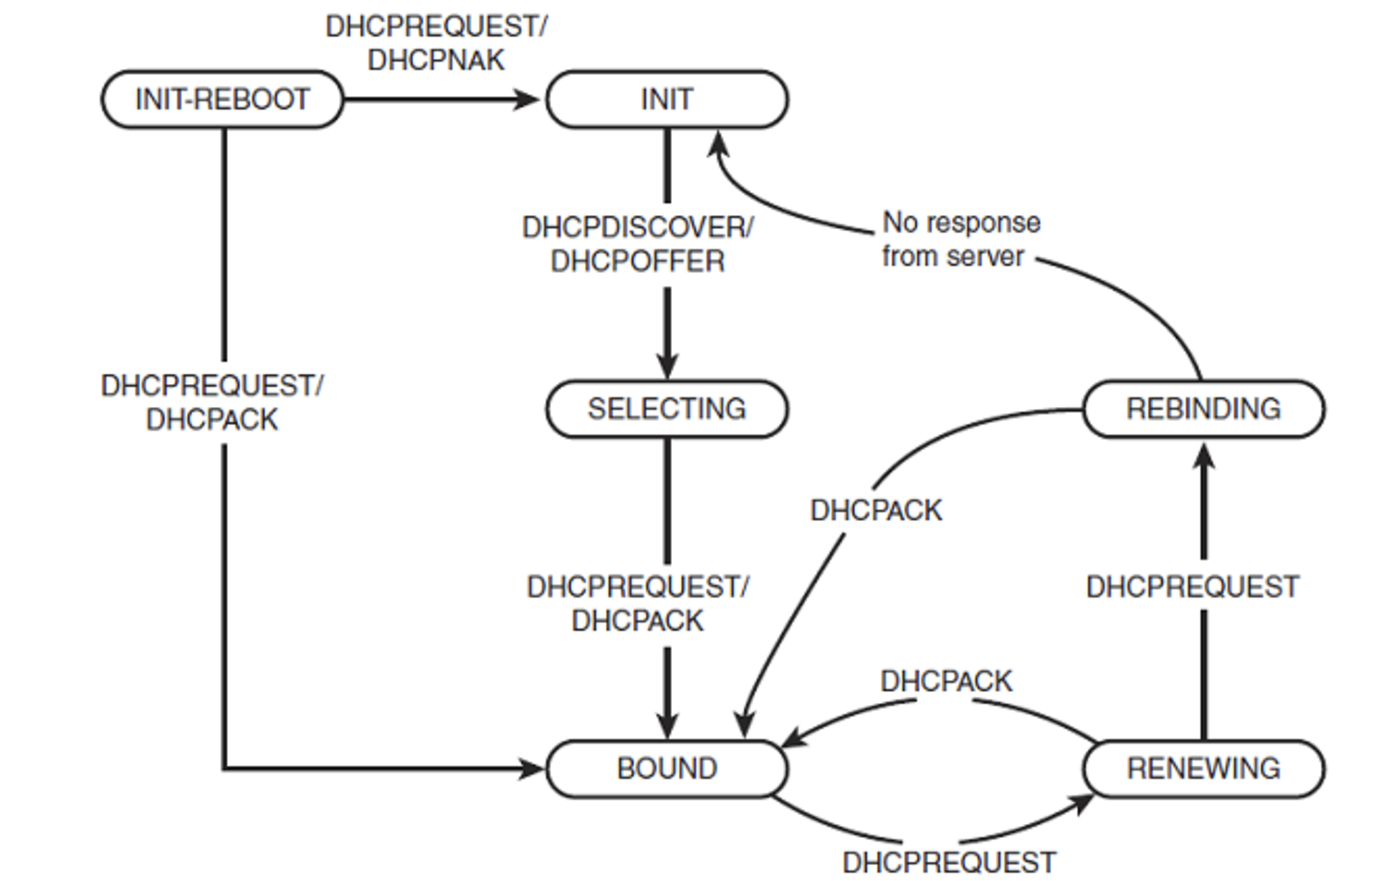
\includegraphics[width=0.7\textwidth]{img/maquinaEstados}
  \caption{Máquina de Estados}
  \label{fig:1}
\end{figure}

Cuando un cliente no tiene una dirección IP válida, se dice que está en el estado INIT. Durante el proceso de configuración inicial, el cliente normalmente se mueve al estado SELECTING, y en el momento en el que está configurado correctamente con una dirección IP, se mueve al estado BOUND. Cuando se reinicia el cliente, se pasa al estado INIT-REBOOT, y después de que se confirma que su dirección IP es válida, se mueve al estado BOUND. Si un servidor envía un mensaje DHCPNAK al cliente, el cliente vuelve al estado INIT.\\\\
Antes de que expire el tiempo de concesión (alquiler, lease) de la dirección IP del cliente, éste entra en estado de RENEWING e intenta extender su contrato de arrendamiento mediante el envío de un mensaje unicast al servidor del que obtuvo su dirección IP. El cliente espera un tiempo, y si no recibe respuesta a su solicitud de renovación, entra en el estado de REBINDING y difunde un mensaje broadcast para extender su contrato de alquiler en cualquier servidor disponible. Si el contrato de arrendamiento expira sin que el cliente renueve con éxito su concesión, el cliente vuelve al estado INIT.\\\\

\subsection{Obtención de la configuración inicial}
	Cuando un equipo configurado para utilizar DHCP se conecta a una red, se determina si tiene una dirección IP válida. Un cliente puede tener una dirección no válida por varios motivos:
	
	\begin{itemize}
		\item Es nuevo y aún no ha recibido nunca una IP.
		\item El tiempo de alquiler de la anterior IP ha expirado.
		\item Un servidor DHCP le dice al cliente que su dirección no es válida (DHCPNACK), normalmente porque se ha movido de segmento de red.
	\end{itemize}

En estos casos, el cliente pasa al estado INIT porque no tiene una dirección válida.\\\\

Cuando el cliente se inicia en el estado INIT, el cliente y el servidor intercambian los siguientes cuatro mensajes:
\begin{itemize}
	\item[\color{airforceblue}DHCPDISCOVER]  El cliente difunde (broadcast) un mensaje DHCPDISCOVER, y el mensaje se entrega a todos los servidores DHCP en el mismo segmento de red del cliente. Este mensaje también es recibido por los agentes de retransmisión del segmento de red del cliente y se reenvía a otros servidores DHCP situados en segmentos de red distintos al del cliente.
	\item[\color{airforceblue}DHCPOFFER] Después de que el servidor recibe el mensaje DHCPDISCOVER desde el cliente, encuentra una dirección para asignar al cliente y la pone en un mensaje DHCPOFFER. El servidor también incluye en este mensaje otros parámetros de configuración, según lo definido por el archivo de configuración del servidor. Después de que el servidor ha completado el mensaje DHCPOFFER, envía el mensaje de vuelta al cliente como broadcast (algunas implementaciones del DHCP lo hace en modo unicast)
	\item[\color{airforceblue}DHCPREQUEST]  Después de que el cliente recibe el(los) mensaje(s) DHCPOFFER, envía un mensaje DHCPREQUEST como broadcast con los datos de la oferta elegida para que el servidor la confirme. Entre estos datos va la dirección del servidor elegido.
	\item[\color{airforceblue}DHCPACK] Después de recibir el mensaje DHCPREQUEST, el servidor comprueba la dirección y los parámetros de configuración requeridos para asegurar que la dirección todavía está disponible y los parámetros son correctos. Registra la dirección asignada y envía el mensaje DHCPACK para que el cliente se configure definitivamente. El cliente cuando recibe este mensaje y se configura, también registra localmente los valores de la concesión. En el caso de que el servidor hubiera asignado la IP a otro cliente antes de recibir el mensaje DHCPREQUEST del primero, se le envía al cliente el mensaje DHCPNACK, rechazando el requerimiento y el cliente vuelve de esta forma al estado INIT. Este mensaje es de tipo broadcast, pero también, igual que sucede con el mensaje DHCPOFFER, algunas implementaciones del servicio DHCP usan tráfico unicast.
\end{itemize}

\begin{figure}
  \centering
    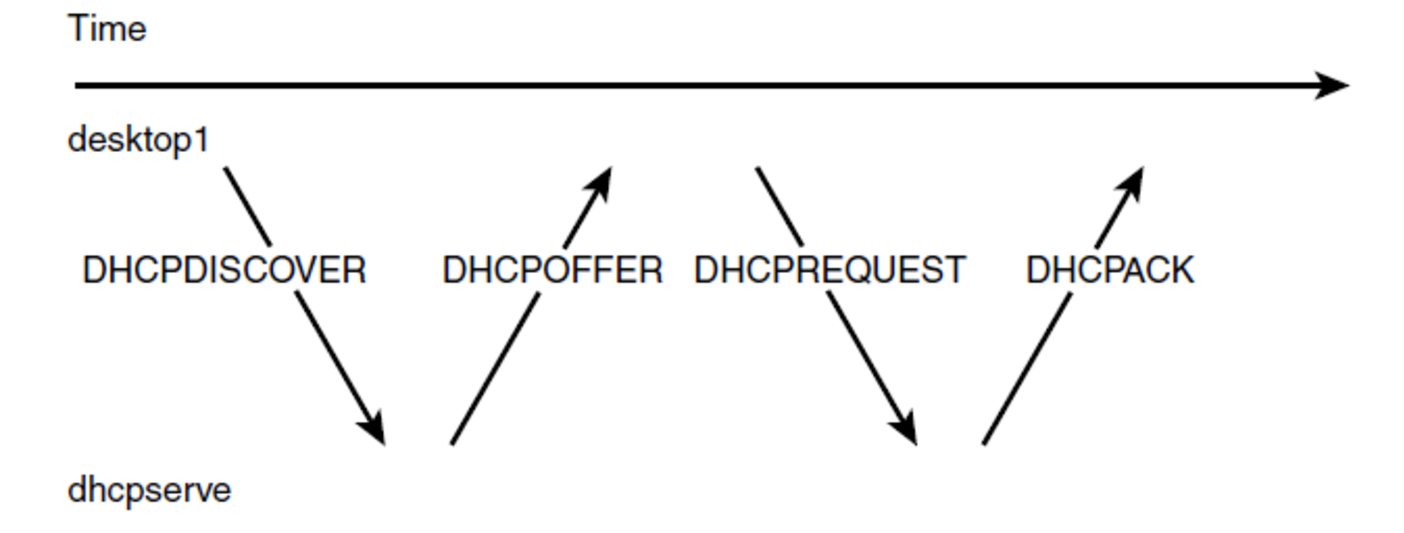
\includegraphics[width=0.7\textwidth]{img/com}
  \caption{Comunicación Cliente-Servidor}
  \label{fig:2}
\end{figure}

En el caso de que hubieran dos servidores DHCP en el mismo segmento de red, el intercambio de mensajes sería como el expuesto en la figura \ref{fig:3}

\begin{figure}
  \centering
    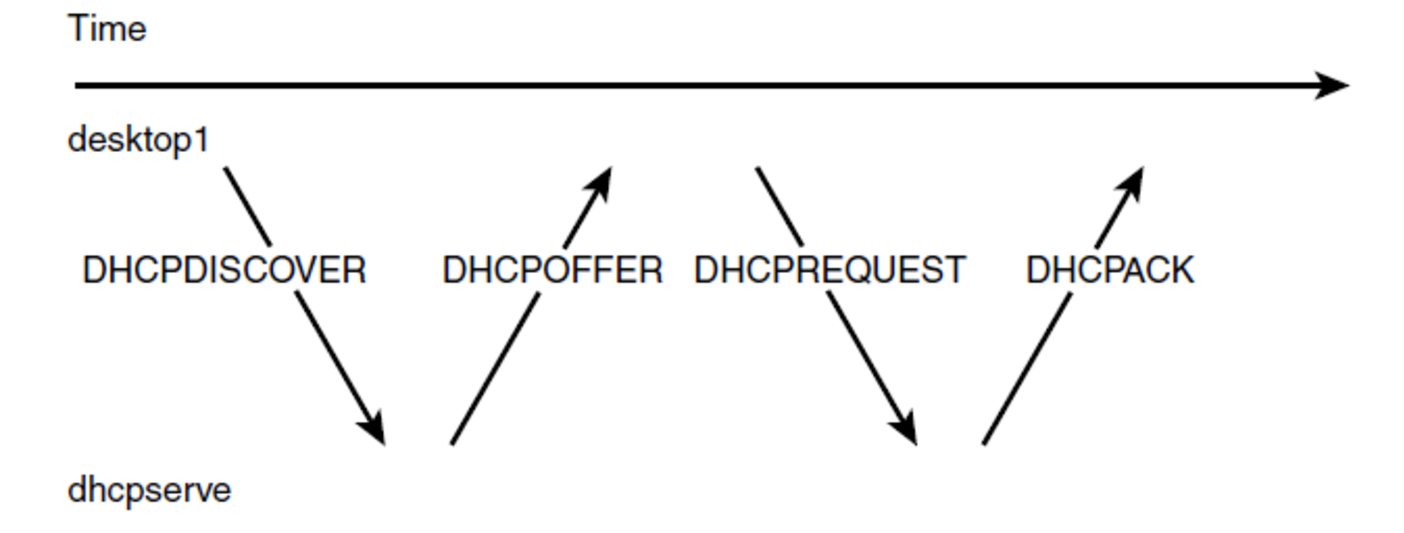
\includegraphics[width=0.7\textwidth]{img/com}
  \caption{Dos servidores}
  \label{fig:3}
\end{figure}

\subsection{Confirmación de Ip tras un reinicio}

Cada vez que se reinicia un cliente, éste comprueba si tiene registrada la dirección IP con un contrato de arrendamiento que aún no haya caducado y en caso afirmativo, se pasa al estado INIT-REBOOT e intenta confirmar que su dirección sigue siendo válida con los siguientes mensajes:
	
	\begin{itemize}
		\item DHCPREQUEST: El cliente envía la dirección IP para ser confirmada en un mensaje DHCPREQUEST como broadcast, el cual es recibido y comprobado por todos los servidores DHCP que están configurados en el segmento de red al que está conectado el cliente. Esta dirección podría no ser válida si el cliente se ha cambiado de segmento de red, o si el administrador de la red ha decidido cambiar el direccionamiento del segmento de red.
		\item Mensaje DHCPACK: Cuando el servidor recibe el mensaje DHCPREQUEST, extrae la dirección solicitada por el cliente y verifica que la dirección es válida y puede utilizarla. Entonces el servidor responde con un mensaje DHCPACK, donde van todos los parámetros de configuración que debe usar el cliente para configurarse. Si el cliente no recibiera respuesta, éste se configurará con la antigua IP siempre que el alquiler no haya expirado.
	\end{itemize}

Algunos clientes DHCP, como por ejemplo el ISC DHCP Client, cuando se para el servicio al apagar el ordenador, envían un mensaje DHCPRELEASE, por lo que liberan su IP y cuando se reinicia el equipo comienzan en el estado INIT enviando un mensaje DHCPDISCOVER.


\section{Implementaciones}
	Todo dispositivo necesita direcciones, isc-dhcp es la opción más eficiente para proveer el servicio. ISC DHCP es código de software abierto como las implementaciones de DNS para conexiones de IP en una red. ISC es una solución que soporta IPv4 y IPv6. DHCP está disponible para descarga gratis bajo sus términos de licencia, con una BSD license.\\\\
	
	Microsoft introdujo el DHCP en sus Servidores NT con la versión 3.5 de Windows NT a finales de 1994.\\\\
	El Consorcio de Software de Internet (ISC: Internet Software Consortium) publicó distribuciones de DHCP para Unix con la versión 1.0.0 del ISC DHCP Server el 6 de diciembre de 1997 y una versión (2.0) que se adaptaba mejor al RFC el día 22 de junio de 1999. Se puede encontrar el software en http://www.isc.org/sw/dhcp/\\\\

Otras implementaciones importantes incluyen:
\begin{itemize}
	\item Cisco: un servidor DHCP habilitado en Cisco IOS 12.0 en el mes de febrero de 1999
	\item Sun: añadió el soporte para DHCP a su sistema operativo Solaris el 8 de julio de 2001.
\end{itemize}

Además, varios routers incluyen soporte DHCP para redes de hasta 255 dispositivos.
%\begin{listing}[style=consola, numbers=none]
%	    $ cd ~/Downloads/
% \end{listing}



%%%%%%%%%% Ejemplo de una tabla %%	
	
%	\begin{table}[h]
%\centering
%\begin{tabular}{l|c|c|c}
%\hline\hline \rowcolor{LightBlue2} Factor a analizar& Peso relativo &Calificación&Calificación ponderada\\ \hline\hline
%\multicolumn{4}{c}{FORTALEZAS}\\ \hline
%F-1& 0.2 		& 4& 0.8 \\
%F-2 & 0.15 & 4& 0.6 \\
%F-3 & 0.1 	& 2&  0.2\\
%F-4 & 0.1 	& 2&  0.2\\
%F-5 & 0.15 & 3&  0.45\\
%F-6 & 0.05 & 2&  0.1\\\hline
%\multicolumn{3}{r}{Total}& 2.35\\ \hline
%\multicolumn{4}{c}{DEBILIDADES}\\ \hline
%D-1& 0.15 & 3& 0.45\\
%D-2 & 0.10 & 2& 0.2\\\hline
%Total&1 & & 0.65\\ \hline
%\end{tabular}
%\caption{MEFI}
%\end{table}